\section{CAPÍTULO III: Propuesta de la solución}

\subsection{3.1 Descripción de la solución}
La solución propuesta consiste en el desarrollo de una aplicación educativa 3D que transforme la experiencia de aprendizaje tradicional mediante la gamificación de tareas académicas en un entorno virtual medieval inmersivo. El sistema integra tecnologías web modernas con estrategias pedagógicas innovadoras para crear un ecosistema educativo que incremente la motivación estudiantil y mejore los resultados de aprendizaje.

La aplicación funcionará como una plataforma integral que conecta docentes, estudiantes y administradores a través de una interfaz web responsiva y aplicaciones móviles. El entorno virtual 3D, desarrollado con Three.js, simula un mundo medieval donde las actividades académicas se transforman en misiones, aventuras y desafíos interactivos que mantienen el engagement estudiantil mientras refuerzan competencias académicas específicas.

El backend se implementará utilizando las API routes de Next.js (con TypeScript) como capa de servidor integrada en la misma aplicación, aprovechando el renderizado híbrido y las ventajas de un único repositorio para cliente y servidor. Estas rutas proporcionarán endpoints para autenticación, administración de usuarios, creación de contenidos gamificados, sistema de evaluaciones y análisis de progreso estudiantil. La base de datos PostgreSQL garantizará la integridad y consistencia de la información educativa, mientras que las integraciones con plataformas existentes como Canvas y Discord ampliarán las capacidades del ecosistema.

\subsubsection{3.1.1 Diagrama de arquitectura}
En el siguiente diagrama se define la arquitectura del proyecto. Se detallan las herramientas empleadas: en el backend, NestJS con TypeScript; en el lado del cliente, React con Three.js para el entorno 3D; como base de datos, PostgreSQL desplegado en servicios cloud (AWS); seguridad mediante JWT integrado con NestJS Guards y autenticación OAuth2 con correo institucional (Google/Microsoft). El sistema incluye integraciones con Canvas LMS y Discord para comunicación, así como un servicio de notificaciones push.

\begin{figure}[H]
	\centering
	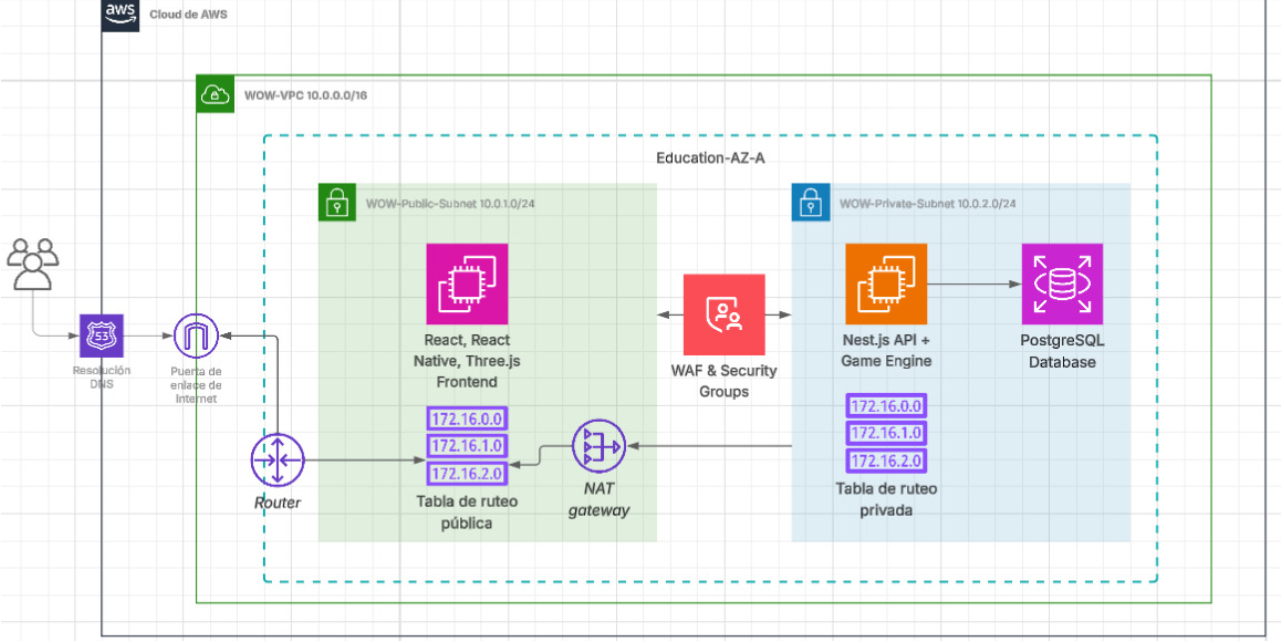
\includegraphics[width=0.95\textwidth]{images/arquitectura.png}
	\caption{Diagrama de arquitectura del proyecto.}
	\label{fig:arquitectura}
\end{figure}

\paragraph{Descripción de componentes principales}
\begin{itemize}
	\item \textbf{Cliente Web (React + Three.js dentro de Next.js)}: Interfaz principal para estudiantes y docentes. Renderiza el entorno 3D y gestiona interacción en tiempo real.
	\item \textbf{API Backend (Next.js API routes)}: Endpoints server-side integrados en Next.js que orquestan la lógica de negocio: autenticación, misiones, evaluación, recompensas y analítica básica.
	\item \textbf{Módulo de Autenticación}: OAuth2 (Google/Microsoft) + JWT (access/refresh) implementado mediante middleware y API routes de Next.js.
	\item \textbf{Base de Datos (PostgreSQL)}: Persistencia relacional: usuarios, cursos, misiones, evaluaciones, progreso, recompensas, avatares.
	\item \textbf{Integraciones Externas}: Canvas (importación/exportación de cursos y calificaciones), Discord (canales de comunicación), Servicio Push (notificaciones de eventos y misiones).
	\item \textbf{Servicio de Analítica}: Procesa eventos de interacción para generar métricas de engagement y rendimiento; puede ejecutarse en serverless functions o microservicios según carga.
	\item \textbf{Orquestación / Infraestructura}: Contenedores Docker para servicios auxiliares y despliegue en Vercel/Cloud (o Kubernetes) para la parte de backend/servicios. El almacenamiento y procesamiento en la nube se realiza exclusivamente en AWS.
\end{itemize}

\subsubsection{3.1.2 Diagramas de Procesos de Negocio (BPMN 2.0)}
Los diagramas BPMN representan el flujo operativo completo del sistema. Capturan la transformación digital de procesos educativos tradicionales, eliminando ineficiencias y habilitando trazabilidad.

\paragraph{Proceso 1: Gestión de Misiones Educativas}
\begin{figure}[H]
	\centering
	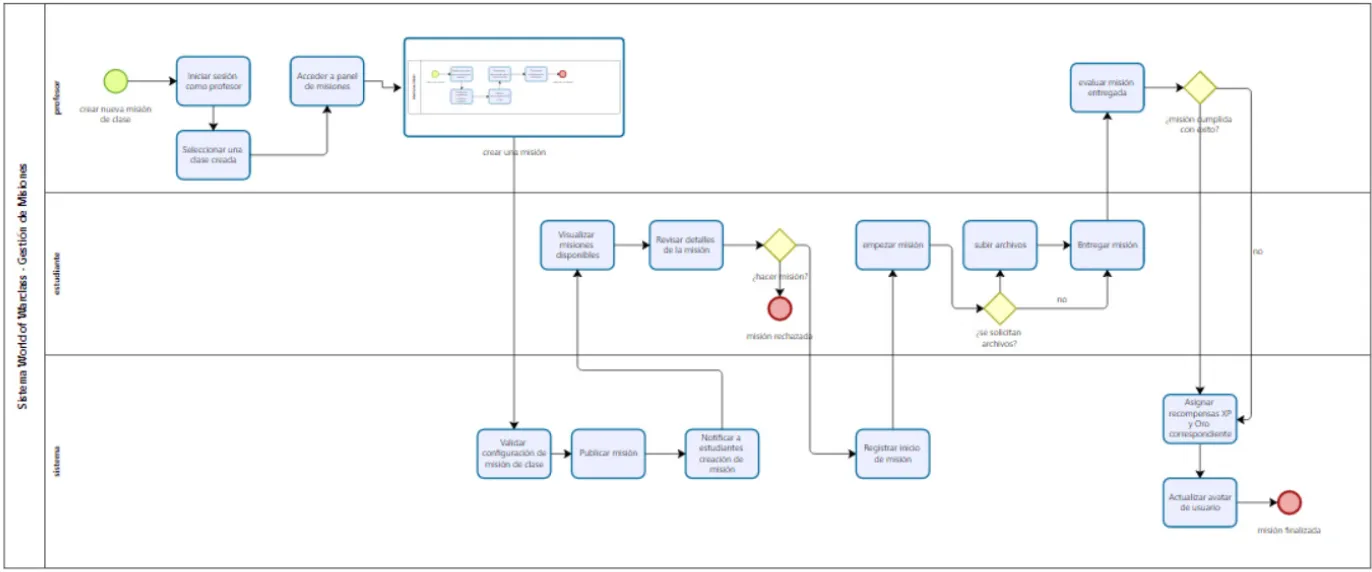
\includegraphics[width=0.95\textwidth]{images/bizgi_gestion_de_misiones.png}
	\caption{Modelo de proceso: Gestión de Misiones Educativas.}
	\label{fig:proc-misiones}
\end{figure}
\textit{Flujo}: Creación de misión (docente) $\rightarrow$ Definición de objetivos y recompensas $\rightarrow$ Publicación $\rightarrow$ Asignación automática/selección $\rightarrow$ Ejecución en entorno 3D $\rightarrow$ Evaluación $\rightarrow$ Retroalimentación y registro de progreso.

\paragraph{Proceso 2: Sistema de Evaluación Gamificada}
\begin{figure}[H]
	\centering
	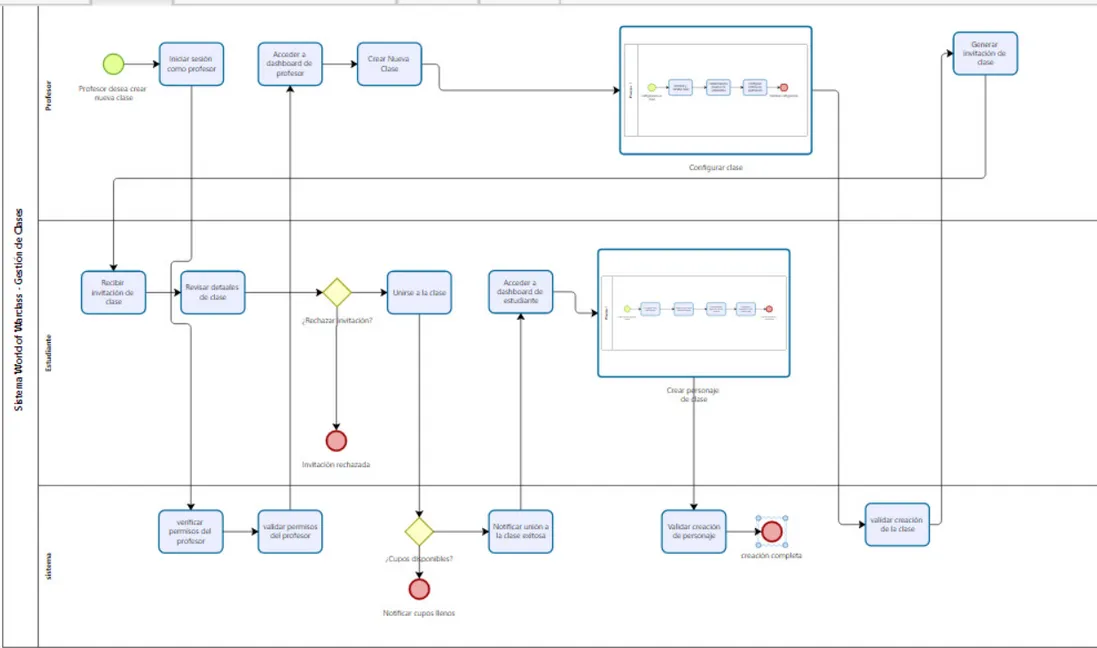
\includegraphics[width=0.95\textwidth]{images/bizagi_gestion_de_clases.png}
	\caption{Modelo de proceso: Sistema de Evaluación Gamificada.}
	\label{fig:proc-evaluacion}
\end{figure}
\textit{Flujo}: Participación estudiante $\rightarrow$ Recolección de métricas $\rightarrow$ Asignación de puntos y logros $\rightarrow$ Actualización de avatar/nivel $\rightarrow$ Registro en base de datos $\rightarrow$ Notificación a docente.

\paragraph{Proceso 3: Análisis y Seguimiento del Progreso}
\begin{figure}[H]
	\centering
	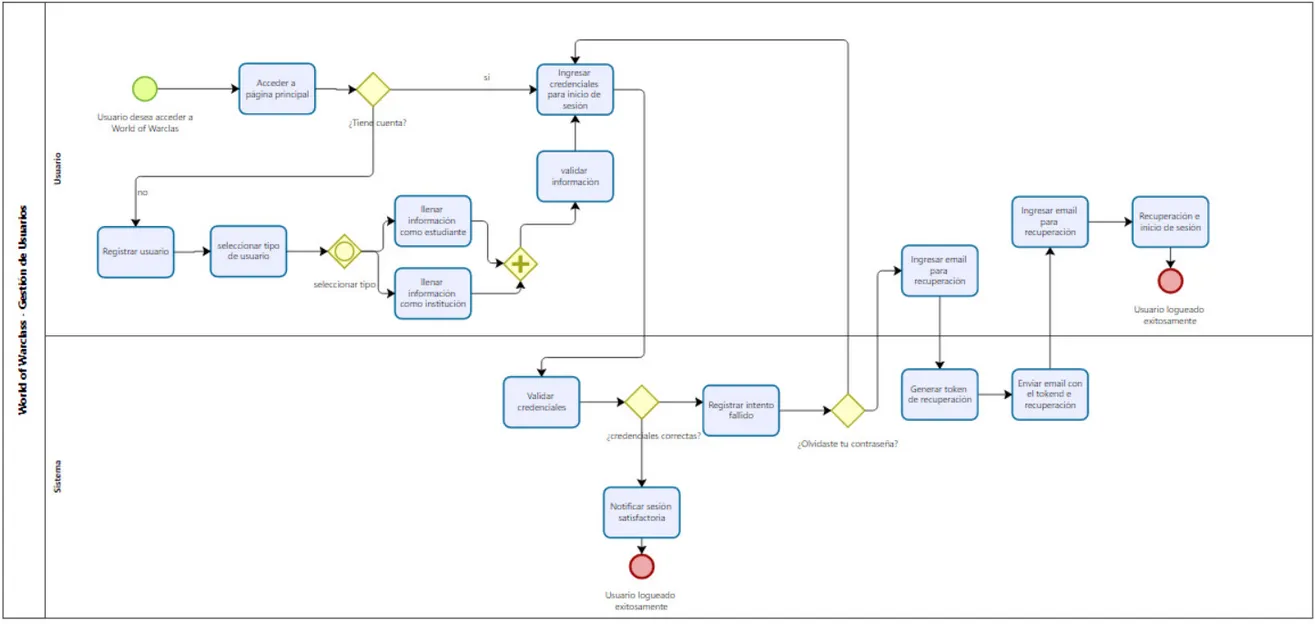
\includegraphics[width=0.95\textwidth]{images/bizagi_gestion_de_usuarios.png}
	\caption{Modelo de proceso: Análisis y Seguimiento del Progreso Estudiantil.}
	\label{fig:proc-analitica}
\end{figure}
\textit{Flujo}: Captura de eventos $\rightarrow$ Almacenamiento $\rightarrow$ Procesamiento analítico $\rightarrow$ Generación de paneles $\rightarrow$ Intervención pedagógica.

\subsubsection{3.1.3 Diagrama Entidad-Relación}
El modelo entidad-relación define las estructuras nucleares para garantizar integridad y trazabilidad.
\begin{figure}[H]
	\centering
	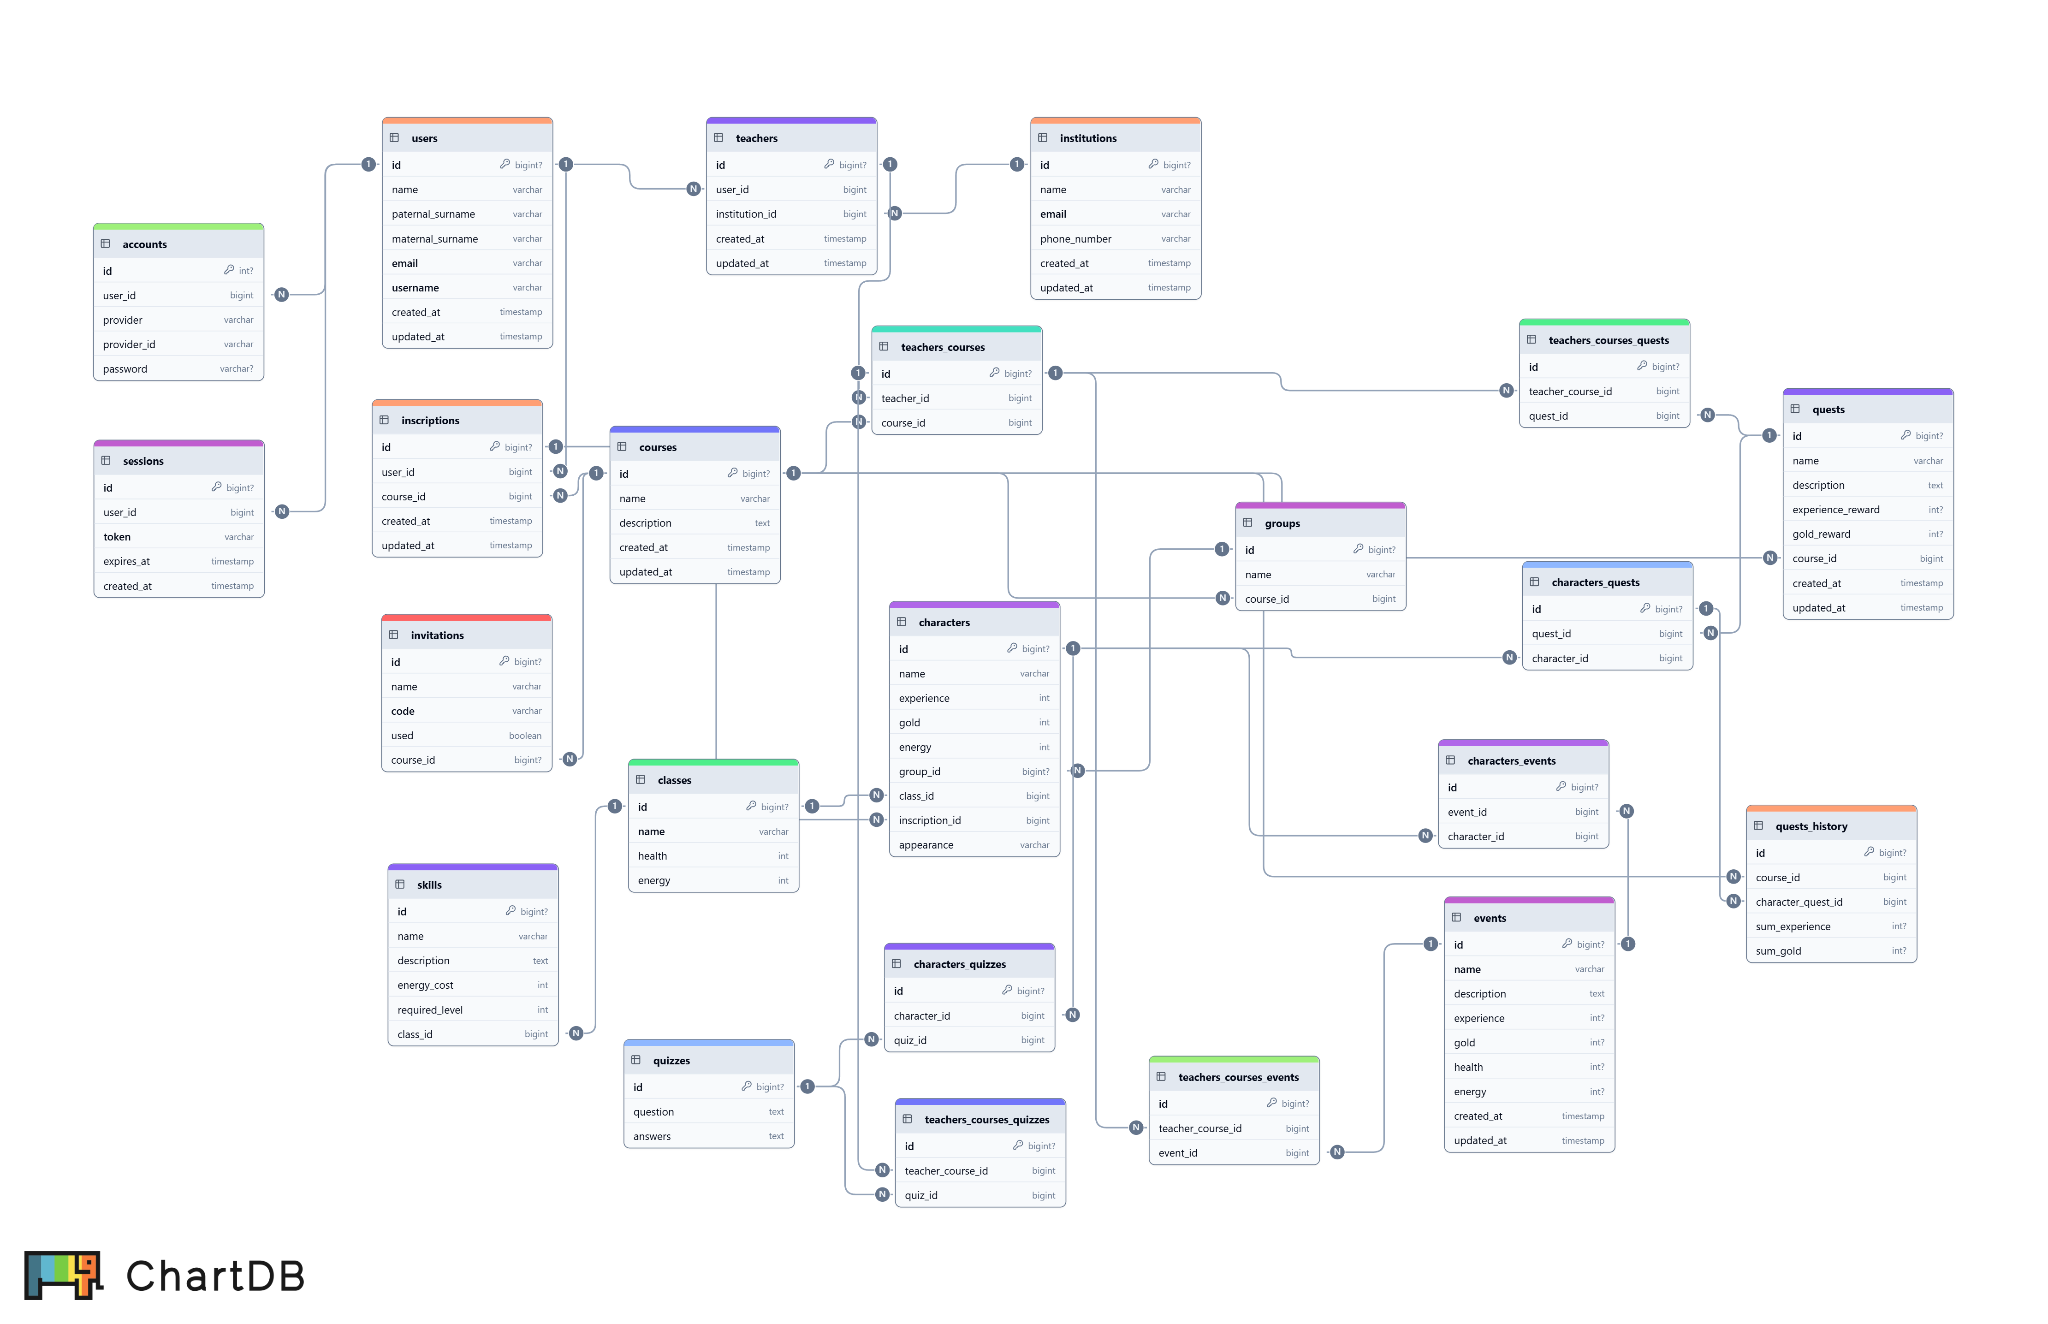
\includegraphics[width=0.95\textwidth]{images/mer.png}
	\caption{Diagrama entidad-relación del sistema.}
	\label{fig:der}
\end{figure}
Entidades principales: Usuarios, Instituciones, Cursos, Misiones, Evaluaciones, Progreso, Recompensas, Avatares. Relaciones jerárquicas permiten seguimiento académico personalizado.

\subsubsection{3.1.4 Prototipo de Interfaces (Figma)}
Las interfaces clave se diseñarán en Figma priorizando usabilidad y consistencia visual.
\begin{figure}[H]
	\centering
	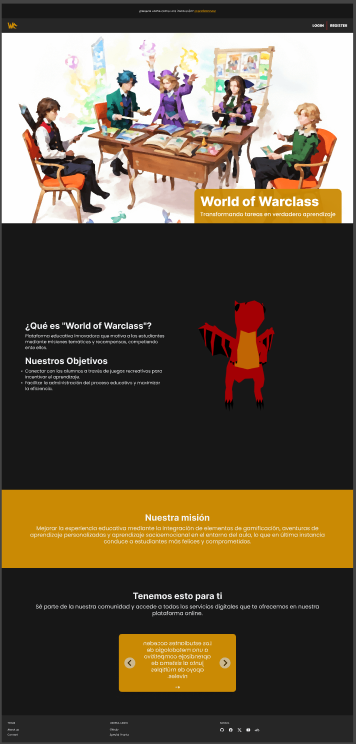
\includegraphics[width=0.75\textwidth]{images/pagina_web_inicio.png}
	\caption{Interfaz principal (home) para usuarios no autenticados.}
	\label{fig:ui-home}
\end{figure}
\begin{figure}[H]
	\centering
	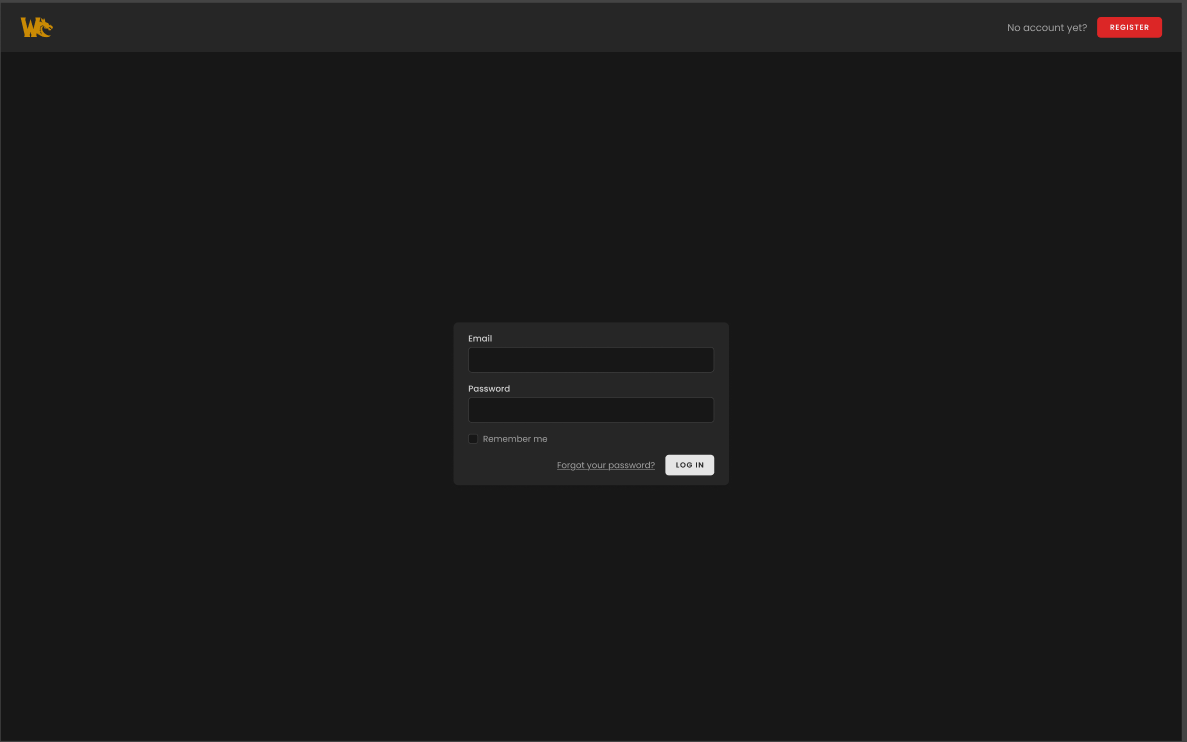
\includegraphics[width=0.75\textwidth]{images/pagina_web_iniciar-sesion.png}
	\caption{Interfaz de Autenticación del proyecto.}
	\label{fig:ui-login}
\end{figure}
\begin{figure}[H]
	\centering
	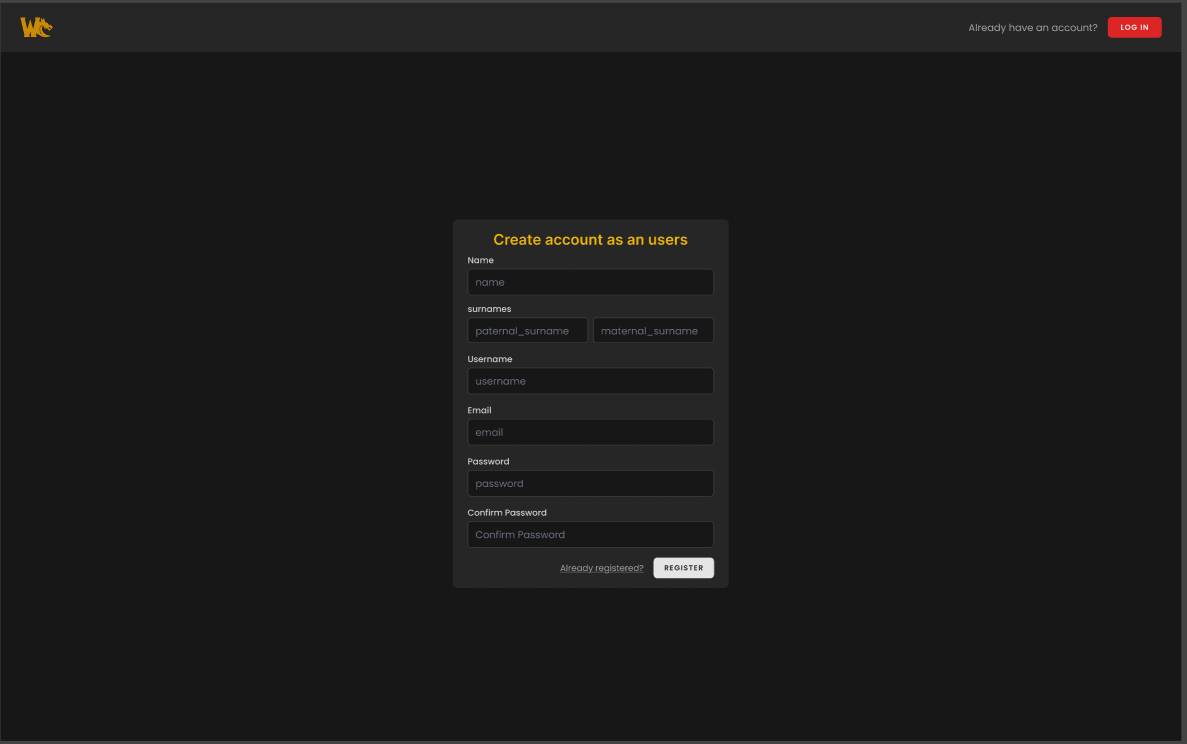
\includegraphics[width=0.75\textwidth]{images/pagina_web_registro.png}
	\caption{Interfaz de Registro de usuario del proyecto.}
	\label{fig:ui-register}
\end{figure}
\begin{figure}[H]
	\centering
	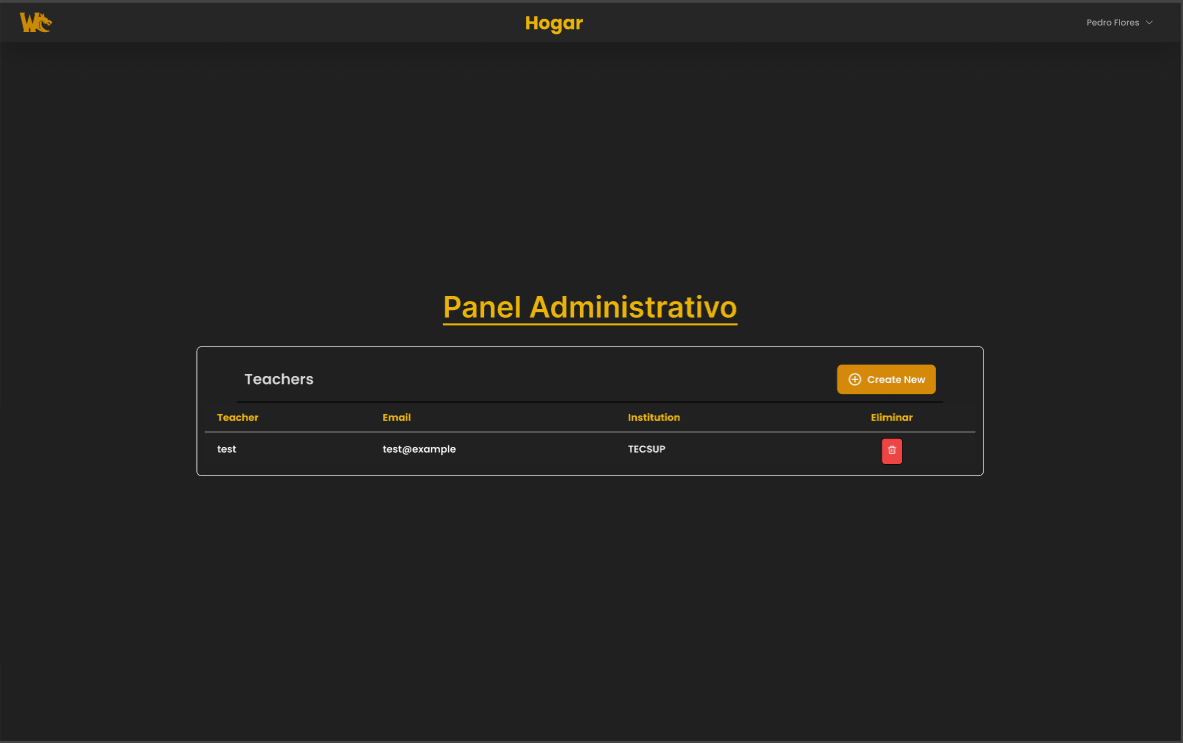
\includegraphics[width=0.75\textwidth]{images/pagina_web_panel-administrativo.png}
	\caption{Interfaz de panel de administración del profesor.}
	\label{fig:ui-profesor}
\end{figure}
\begin{figure}[H]
	\centering
	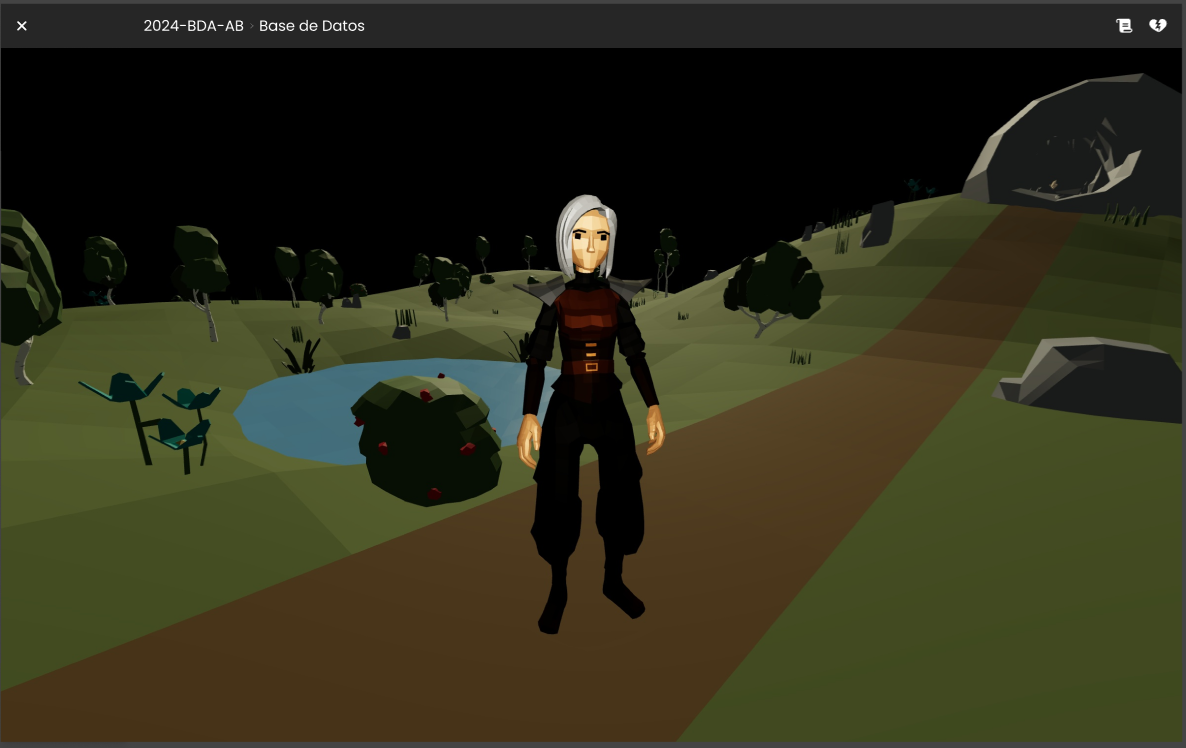
\includegraphics[width=0.75\textwidth]{images/pagina_web_vista-alumno.png}
	\caption{Gestión de avatar del estudiante.}
	\label{fig:ui-avatar}
\end{figure}

\subsection{3.2 Descripción de la metodología de desarrollo de software}
La metodología seleccionada para el proyecto es \textbf{Kanban} (marco ágil de flujo continuo) complementada con prácticas de integración continua y despliegue continuo (CI/CD). Se eligió debido a que el equipo es muy pequeño (2 personas) y varios integrantes trabajan en sus tiempos libres; Kanban reduce la sobrecarga de ceremonias y facilita el flujo de trabajo mediante un tablero visual y límites de trabajo en curso (WIP).

\subsubsection{3.2.1 Justificación de la selección de Kanban}
\begin{itemize}
	\item \textbf{Equipo pequeño y disponibilidad limitada}: con solo dos personas y trabajo a tiempo parcial, Kanban minimiza reuniones y coordinación pesada.
	\item \textbf{Flujo continuo}: permite priorizar y avanzar tareas según la capacidad real del equipo sin forzar iteraciones fijas.
	\item \textbf{Menor overhead administrativo}: no requiere ceremonias formales obligatorias (planning, sprint review, retro) lo que ahorra tiempo en proyectos con recursos limitados.
	\item \textbf{Visualización y control de WIP}: el tablero Kanban facilita identificar cuellos de botella, visualizar el progreso y limitar el trabajo en curso para mejorar el flujo.
\end{itemize}

\subsubsection{3.2.2 Épicas e Historias de Usuario}
Las épicas agrupan funcionalidades estratégicas. A continuación se muestran épicas con ejemplos de historias asociadas:

\begin{table}[ht]
	\centering
	\caption{Épicas e historias de usuario (Tabla 14).}
	\begin{tabular}{p{3cm} p{10cm}}
		\toprule
		Épica & Historias (resumen) \\
		\midrule
		Autenticación & Como estudiante quiero registrarme con mi cuenta institucional para acceder a mis cursos.\\
		Misiones & Como docente quiero crear una misión con objetivos y recompensas para motivar a mis alumnos.\\
		Evaluación & Como docente quiero ver el rendimiento agregado de una misión para ajustar la dificultad.\\
		Progreso & Como estudiante quiero visualizar mi nivel y logros para entender mi avance.\\
		Analítica & Como administrador quiero paneles de uso para evaluar adopción y engagement.\\
		Integraciones & Como docente quiero importar calificaciones desde Canvas para unificar seguimiento.\\
		Notificaciones & Como estudiante quiero recibir avisos cuando haya nuevas misiones disponibles.\\
		\bottomrule
	\end{tabular}
\end{table}

\begin{figure}[H]
	\centering
	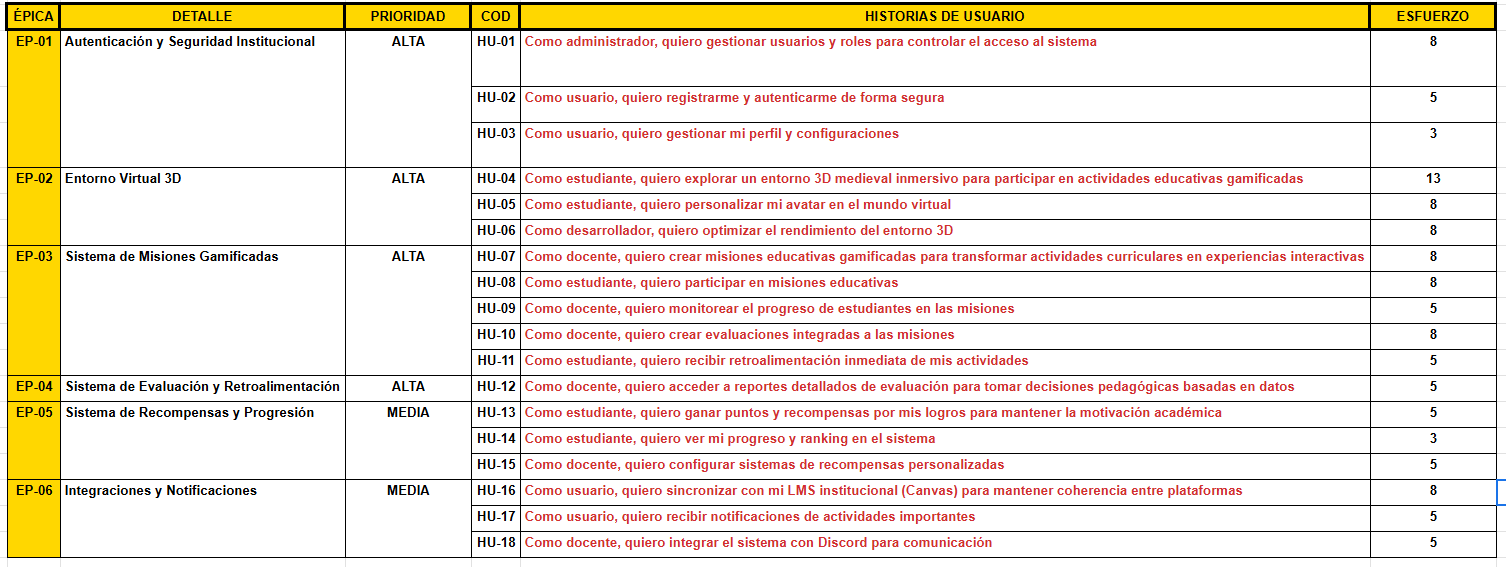
\includegraphics[width=0.85\textwidth]{images/epicas.png}
	\caption{Diagrama de épicas del proyecto.}
	\label{fig:epicas}
\end{figure}

\begin{figure}[H]
	\centering
	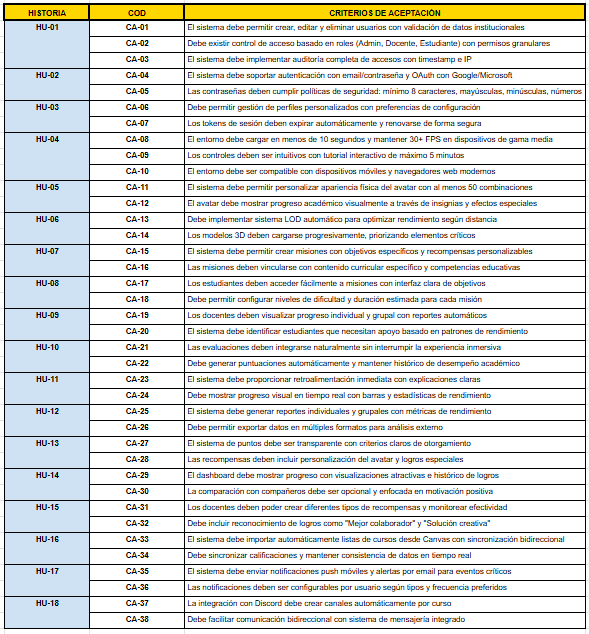
\includegraphics[width=0.85\textwidth]{images/historias_de_usuario.png}
	\caption{Historias de usuario detalladas por épica.}
	\label{fig:historias-usuario}
\end{figure}

\subsubsection{3.2.3 Criterios de aceptación}
Ejemplos de criterios asociados a historias clave:
\begin{itemize}
	\item Autenticación: flujo completo OAuth2 + JWT, expiración configurable, refresco transparente.
	\item Creación de misión: validación de campos obligatorios, guardado atómico, versionado de cambios.
	\item Evaluación automática: registro de puntuación y tiempo, asignación de recompensas según umbrales.
	\item Progreso visual: actualización en tiempo real del nivel tras recibir puntos.
	\item Analítica: métricas mínimas (tiempo activo, misiones completadas, ratio abandono) exportables en CSV.
\end{itemize}

\begin{table}[ht]
	\centering
	\caption{Criterios de aceptación por historia (Tabla 15).}
	\begin{tabular}{p{3.2cm} p{9.8cm}}
		\toprule
		Historia & Criterios (resumen) \\
		\midrule
		Registro & Email institucional verificado, password seguro, confirmación por enlace.\\
		Login & Token válido emitido, revocación en logout, bloqueo tras intentos fallidos.\\
		Crear misión & Objetivos >=1, recompensa asignada, retroalimentación opcional, estado inicial Borrador.\\
		Completar misión & Cambia estado a Completada, asigna puntos y XP, registra timestamp.\\
		Ver progreso & Muestra nivel, XP restante, logros recientes y próximas recompensas.\\
		Panel analítica & Filtra por curso, fecha y tipo de misión; exporta reporte.\\
		Notificación & Envío push dentro de 10s tras publicación de misión.\\
		\bottomrule
	\end{tabular}
\end{table}

\subsection{3.3 Planificación (Gantt)}
El diagrama de Gantt representa la programación de actividades a lo largo del tiempo, mostrando duración, secuencia y dependencias. El proyecto se planifica en 24 semanas distribuidas en seis fases estratégicas.
\begin{itemize}
	\item \textbf{Fase 1 (Sem 1-4) Análisis y Diseño}: requisitos, stakeholders, historias, arquitectura, DER.
		\item \textbf{Fase 2 (Sem 5-10) Backend / API}: implementación de Next.js API routes con TypeScript, autenticación, gestión de usuarios, endpoints para misiones, evaluación automática e integraciones con LMS.
	\item \textbf{Fase 3 (Sem 11-16) Frontend}: interfaz React, entorno 3D, dashboard, app móvil, avatares.
	\item \textbf{Fase 4 (Sem 17-20) Módulos y Analítica}: algoritmos de engagement, detección de anomalías, personalización.
	\item \textbf{Fase 5 (Sem 21-22) Testing}: pruebas integración, seguridad, rendimiento, usabilidad.
	\item \textbf{Fase 6 (Sem 23-24) Despliegue y Capacitación}: infraestructura cloud, CI/CD, formación docente.
\end{itemize}

\begin{figure}[H]
	\centering
	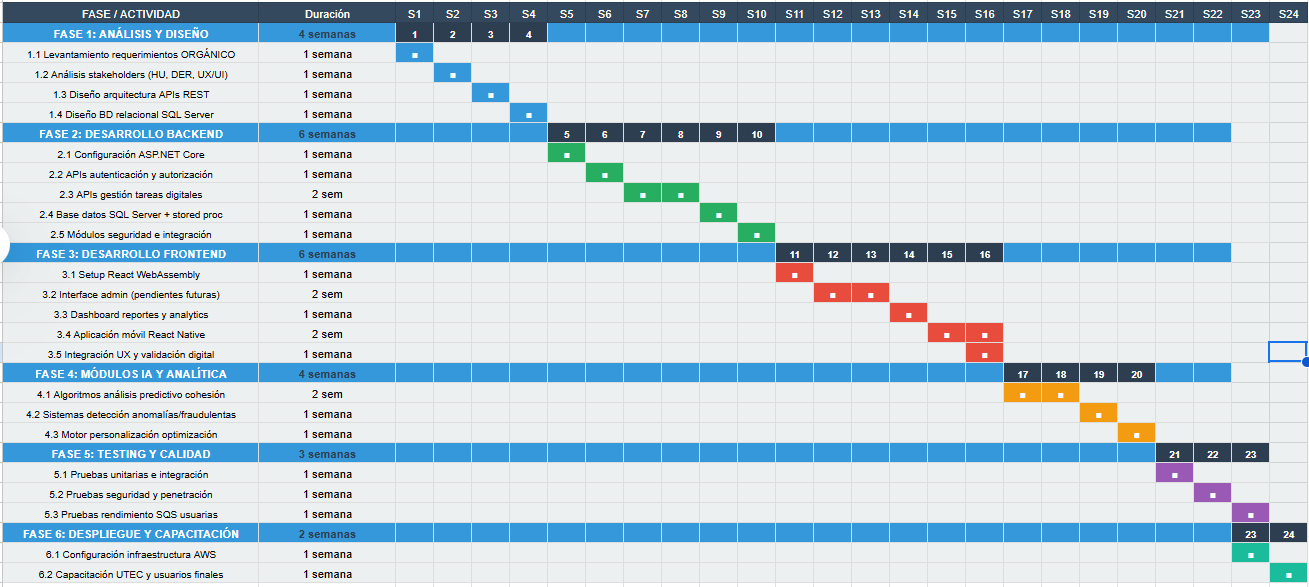
\includegraphics[width=0.95\textwidth]{images/gantt.png}
	\caption{Diagrama de Gantt del proyecto.}
	\label{fig:gantt}
\end{figure}
